%%%%%%%%%%%%%%%%%%%%%%%%%%%%%%%%%%%%%%%%%%%%%%%%%%%%%%%%%%%%%%%
%
% Welcome to Overleaf --- just edit your LaTeX on the left,
% and we'll compile it for you on the right. If you open the
% 'Share' menu, you can invite other users to edit at the same
% time. See www.overleaf.com/learn for more info. Enjoy!
%
%%%%%%%%%%%%%%%%%%%%%%%%%%%%%%%%%%%%%%%%%%%%%%%%%%%%%%%%%%%%%%%
\documentclass{slides}

% if using pdflatex

\usepackage[utf8]{inputenc}

% \usepackage[T1]{fontenc}

\usepackage[scaled=0.85]{roboto-mono}
\usepackage{epigraph} 
\usepackage{listings}
\usepackage{cancel}
\usepackage{subfig}

\usepackage{graphicx}
\graphicspath{{images/}}
%Information to be included in the title page:
\title{Rust 101 - Lecture 2}
\author{Jordan Hall}
\institute{DoCSoc}
\date{2022}

\newcommand{\centerimg}[2]{
    \begin{center}
        \includegraphics[#1]{#2}
    \end{center}
}

\begin{document}

\frame{\titlepage}

\begin{frame}
\frametitle{Roadmap}
\centerimg{width=10cm}{roadmap}
\end{frame}

\begin{frame}
\frametitle{Before We Start}
The slides are now over on my GitHub page (so you can make notes):

\href{https://github.com/JordanLloydHall/RustCourse}{https://github.com/JordanLloydHall/RustCourse}
\end{frame}

\begin{frame}
\frametitle{Quick Recap}
Last time we took a look at variables, basic types, control flow, and functions.
Most of these ideas are not particularly new. They look similar to structures of other languages.
But then we came across something weird:
\end{frame}

\begin{frame}[fragile]
\frametitle{A Problem with Functions (continued)}
\begin{minted}[fontsize=\footnotesize]{rust}
fn length_of_username(user: User) -> usize {
    user.username.len()
}
fn main() {
    let tony = User {
        active: false,
        username: String::from("Tony"),
        email: String::from("OohBaby42@haskell.org"),
        sign_in_count: 12345
    };
    let l = length_of_username(tony);
    assert_eq!(4, l);
    assert!(!tony.active)
}
\end{minted}
\end{frame}

\begin{frame}[fragile]
\frametitle{A Problem with Functions (continued)}
\begin{minted}[fontsize=\footnotesize]{rust}
error[E0382]: use of moved value: `tony`
  --> src/main.rs:20:14
   |
12 |     let tony = User {
   |         ---- move occurs because `tony` has type `User`, which does not implement 
   |                the `Copy` trait
...
18 |     let l = length_of_username(tony);
   |                                ---- value moved here
19 |     assert_eq!(4, l);
20 |     assert!(!tony.active)
   |              ^^^^^^^^^^^ value used here after move

For more information about this error, try `rustc --explain E0382`.
\end{minted}
\end{frame}

\begin{frame}[fragile]
\frametitle{Borrows and Ownership}
\begin{minted}[fontsize=\footnotesize]{rust}
fn length_of_username(user: &User) -> usize {
    user.username.len()
}
fn main() {
    let tony = User {
        active: false,
        username: String::from("Tony"),
        email: String::from("OohBaby42@haskell.org"),
        sign_in_count: 12345
    };
    let l = length_of_username(&tony);
    assert_eq!(4, l);
    assert!(!tony.active)
}
\end{minted}
\end{frame}

\begin{frame}[fragile]
\frametitle{Borrows and Ownership (continued)}
Without the reference, we had the following flow diagram:
\centerimg{width=9cm}{ownership}

With the reference, we had the following flow diagram:
\centerimg{width=9cm}{mutable_borrow}
\end{frame}

\begin{frame}[fragile]
\frametitle{Borrows and Ownership}
\begin{minted}[fontsize=\footnotesize]{rust}
fn sign_in_user(user: &mut User) {
    user.sign_in_count += 1;
    user.active = true;
}
fn main() {
    let mut tony = User {
        active: false,
        username: String::from("Tony"),
        email: String::from("OohBaby42@haskell.org"),
        sign_in_count: 12345
    };
    sign_in_user(&mut tony);
    assert_eq!(12346, tony.sign_in_count);
    assert!(tony.active);
}
\end{minted}
\end{frame}

\begin{frame}
\frametitle{Borrow Hierarchy}
\begin{figure}%
    \centering
    \subfloat{{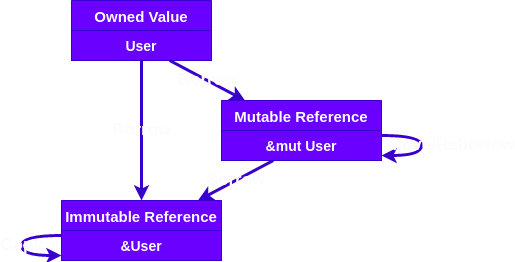
\includegraphics[width=7cm]{borrow_hirarchy2} }}%
    \qquad
    \subfloat{{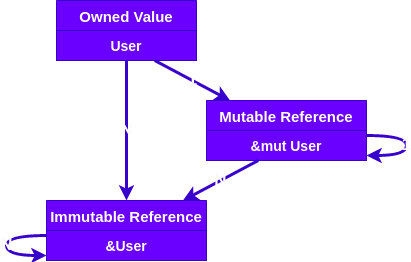
\includegraphics[width=6cm]{borrow_hirearchy} }}%
    \label{fig:example}%
\end{figure}
% \centerimg{width=5.5cm}{borrow_hirarchy2}
Questions:
\begin{enumerate}
    \item Why can't you have more than one mutable reference at the same time?
    \item Why can't an immutable reference create a mutable reference?
    \item Why can a mutable reference create immutable references, but a owned value can't create both a mutable and immutable reference at the same time?
\end{enumerate}
\end{frame}

\begin{frame}[fragile]
\frametitle{Borrow Hierarchy (continued)}
\begin{minted}[]{rust}
fn main() {
    let s = String::from("It's Over, Anakin. I Have The High Ground");

    let ref1: &String = &s;
    let ref2: &String = ref1;

    println!("{}\n{}", ref1, ref2);
}
\end{minted}
Questions:
\begin{enumerate}
    \item Does this code compile?
    \item If not, why?
\end{enumerate}
\end{frame}

\begin{frame}[fragile]
\frametitle{Borrow Hierarchy (continued)}
\begin{minted}[]{rust}
fn main() {
    let s = String::from("It's Over, Anakin. I Have The High Ground");

    let ref1: &String = &s;

    println!("{}\n{}\n{}", ref1, s);
}
\end{minted}
Questions:
\begin{enumerate}
    \item Does this code compile?
    \item If not, why?
\end{enumerate}
\end{frame}

\begin{frame}[fragile]
\frametitle{Borrow Hierarchy (continued)}
\begin{minted}[]{rust}
fn main() {
    let mut s = String::from("It's Over, Anakin. I Have The High Ground");

    let mut_ref: &mut String = &mut s;
    let immut_ref: &String = &s;
    
    println!("{}\n{}", mut_ref, immut_ref);
}
\end{minted}
Questions:
\begin{enumerate}
    \item Does this code compile?
    \item If not, why?
\end{enumerate}
\end{frame}

\begin{frame}[fragile]
\frametitle{Borrow Hierarchy (continued)}
\begin{minted}[fontsize=\footnotesize]{rust}
error[E0502]: cannot borrow `s` as immutable because it is also borrowed as mutable
  --> src/main.rs:16:30
   |
15 |     let mut_ref: &mut String = &mut s;
   |                                ------ mutable borrow occurs here
16 |     let immut_ref: &String = &s;
   |                              ^^ immutable borrow occurs here
17 |     
18 |     println!("{}\n{}", mut_ref, immut_ref);
   |                        ------- mutable borrow later used here

For more information about this error, try `rustc --explain E0502`.
\end{minted}
\end{frame}

\begin{frame}[fragile]
\frametitle{Strings!}
\begin{minted}[]{rust}
fn main() {
    let s1: &str = "Hello World!";
    let s2: &str = &s1[..5];
    println!("{}, {}", s1, s2);
}
\end{minted}
\end{frame}

\begin{frame}
\section{Traits}
\end{frame}

% \begin{frame}
% \section{\xcancel{Traits} Object Oriented Programming was a mistake}
% \end{frame}

\begin{frame}[fragile]
\frametitle{What Traits are}
Traits are a collection of methods that can be called on things that implement them.

They describe what a type with that trait is able to do.
\end{frame}


\begin{frame}[fragile]
\frametitle{First Look at Traits}
\begin{minted}[]{rust}
struct User {
    active: bool,
    username: String,
    email: String,
    sign_in_count: u64,
}
\end{minted}
\end{frame}

\begin{frame}[fragile]
\frametitle{First Look at Traits (continued)}
\begin{minted}[]{rust}
impl User {
    fn login(&mut self) -> bool {
        if self.active {
            false
        } else {
            self.sign_in_count += 1;
            self.active = true;
            true
        }
    }
...
\end{minted}
\end{frame}

\begin{frame}[fragile]
\frametitle{First Look at Traits (continued)}
\begin{minted}[]{rust}
...
    fn logout(&mut self) -> bool {
        if self.active {
            self.active = false;
            true
        } else {
            false
        }
    }
}
...
\end{minted}
\end{frame}

\begin{frame}[fragile]
\frametitle{First Look at Traits (continued)}
\begin{minted}[]{rust}
...
fn main() {
    let mut tony = User {
        active: true,
        username: String::from("Tony"),
        email: String::from("OohBaby42@haskell.org"),
        sign_in_count: 12345
    };
    tony.logout();
    tony.login();
    assert!(tony.active);
    assert_eq!(tony.sign_in_count, 12346);
}
\end{minted}
\end{frame}

\begin{frame}[fragile]
\frametitle{First Look at Traits (continued)}
\begin{minted}[fontsize=\scriptsize]{rust}
impl User {
    fn login(&mut self) -> bool {
        if self.active {
            false
        } else {
            self.sign_in_count += 1;
            self.active = true;
            true
        }
    }
    fn logout(&mut self) -> bool {
        if self.active {
            self.active = false;
            true
        } else {
            false
        }
    }
}
\end{minted}
\end{frame}

\begin{frame}[fragile]
\frametitle{A Second Look at Traits}
\begin{minted}[fontsize=\footnotesize]{rust}
trait Quote {
    fn quote(&self) -> String;
}

struct MaceWindu;
struct Tony;

impl Quote for MaceWindu {
    fn quote(&self) -> String {
        String::from("You are on this council, but we do not grant you the rank of Master.")
    }
}
impl Quote for Tony {
    fn quote(&self) -> String {
        String::from("Ohhhhhhh baby!")
    }
}
\end{minted}
\end{frame}

\begin{frame}[fragile]
\frametitle{A Second Look at Traits (continued)}
\begin{minted}[fontsize=\footnotesize]{rust}
fn main() {
    let windu = MaceWindu;
    let tony = Tony;

    assert_eq!(
        windu.quote(),
        String::from("You are on this council, but we do not grant you the rank of Master.")
    );
    assert_eq!(tony.quote(), String::from("Ohhhhhhh baby!"));
}
\end{minted}
\end{frame}

\begin{frame}[fragile]
\frametitle{Using Traits in Functions}
\begin{minted}[]{rust}
fn print_quote_long<T: Quote>(quoter: &T) {
    println!("{}", quoter.quote());
}
fn print_quote_short(quoter: &impl Quote) {
    println!("{}", quoter.quote());
}
fn main() {
    let windu = MaceWindu;
    print_quote_long(&windu);
    print_quote_short(&windu);
}
\end{minted}
\end{frame}

\begin{frame}[fragile]
\frametitle{More Than One Trait}
\begin{minted}[fontsize=\footnotesize]{rust}
trait Name {
    fn name(&self) -> String;
}
impl Name for MaceWindu {
    fn name(&self) -> String {
        String::from("Mace Windu (Jedi Master)")
    }
}
fn print_quote<T: Name + Quote>(quoter: &T) {
    println!("{} - {}", quoter.quote(), quoter.name())
}
fn main() {
    let windu = MaceWindu;
    let tony = Tony;
    print_quote(&windu);
}
\end{minted}
\end{frame}

\begin{frame}[fragile]
\frametitle{More Than One Trait (continued)}
\begin{minted}[fontsize=\small]{rust}
trait Name {
    fn name(&self) -> String;
}
fn print_quote<T: Name + Quote>(quoter: &T) {
    println!("{} - {}", quoter.quote(), quoter.name())
}
fn main() {
    let tony = Tony;
    print_quote(&tony);
}
\end{minted}
\end{frame}


\begin{frame}[fragile]
\frametitle{More Than One Trait (continued)}
\begin{minted}[fontsize=\small]{rust}
error[E0277]: the trait bound `Tony: Name` is not satisfied
  --> src/main.rs:32:17
   |
32 |     print_quote(&tony);
   |     ----------- ^^^^^ the trait `Name` is not implemented for `Tony`
   |     |
   |     required by a bound introduced by this call
   |
note: required by a bound in `print_quote`
  --> src/main.rs:26:19
   |
26 | fn print_quote<T: Name + Quote>(quoter: &T) {
   |                   ^^^^ required by this bound in `print_quote`

For more information about this error, try `rustc --explain E0277`.
\end{minted}
\end{frame}

\begin{frame}[fragile]
\frametitle{More Than One Trait (continued)}
\begin{minted}[fontsize=\small]{rust}
fn print_quote<T: Name + Quote>(quoter: &T) {
    println!("{} - {}", quoter.quote(), quoter.name())
}

fn print_quote<T>(quoter: &T)
where
    T: Name + Quote,
{
    println!("{} - {}", quoter.quote(), quoter.name())
}
\end{minted}
\end{frame}

\begin{frame}[fragile]
\frametitle{Supertraits}
\begin{minted}[]{rust}
trait Name {
    fn name(&self) -> String;
}
trait Quote: Name {
    fn quote(&self) -> String;
    fn speak(&self) {
        println!("{} says {}", self.name(), self.quote())
    }
}
\end{minted}
\end{frame}

\begin{frame}[fragile]
\frametitle{Supertraits (continued)}
\begin{minted}[]{rust}
struct Dog;
impl Name for Dog {
    fn name(&self) -> String {
        String::from("Dog")
    }
}
impl Quote for Dog {
    fn quote(&self) -> String {
        String::from("Wooof!")
    }
}
\end{minted}
\end{frame}

\begin{frame}[fragile]
\frametitle{Supertraits (continued)}
\begin{minted}[]{rust}
fn main() {
    let dog = Dog;
    dog.speak();
}
\end{minted}
\end{frame}

\begin{frame}[fragile]
\frametitle{Supertraits (continued)}
\begin{minted}[]{rust}
struct Cat;
impl Quote for Cat {
    fn quote(&self) -> String {
        String::from("Meow")
    }
}
\end{minted}
\end{frame}

\begin{frame}[fragile]
\frametitle{Supertraits (continued)}
\begin{minted}[]{rust}
error[E0277]: the trait bound `Cat: Name` is not satisfied
  --> src/main.rs:11:6
   |
11 | impl Quote for Cat {
   |      ^^^^^ the trait `Name` is not implemented for `Cat`
   |
note: required by a bound in `Quote`
  --> src/main.rs:4:14
   |
4  | trait Quote: Name {
   |              ^^^^ required by this bound in `Quote`

For more information about this error, try `rustc --explain E0277`.
\end{minted}
\end{frame}

\begin{frame}[fragile]
\frametitle{Constant Generics}
We have already seen the most basic use of constant generics.
They allow an integer to be a part of a type, known at compile-time.

\begin{minted}[]{rust}
let xs: [i32; 5] = [1, 2, 3, 4, 5];
\end{minted}
\end{frame}

\begin{frame}[fragile]
\frametitle{Constant Generics (continued)}
\begin{minted}[]{rust}
fn cumulate<const N: usize>(mut arr: [i32; N]) -> [i32; N] {
    let mut sum = 0;
    for i in 0..N {
        sum += arr[i];
        arr[i] = sum;
    }
    arr
}
fn main() {
    let arr = cumulate([1; 10]);
    assert_eq!(arr, [1, 2, 3, 4, 5, 6, 7, 8, 9, 10]);
}
\end{minted}
\end{frame}

\begin{frame}[fragile]
\frametitle{A Problem With References}
\begin{minted}[]{rust}
fn return_slice(s: &str) -> &str {
    &s[..5]
}
fn main() {
    assert_eq!(return_slice("Hello World!"), "Hello")
}
\end{minted}
\end{frame}

\begin{frame}[fragile]
\frametitle{A Problem With References (continued)}
\begin{minted}[]{rust}
fn return_largest_str(s1: &str, s2: &str) -> &str {
    if s1.len() >= s2.len() {
        s1
    } else {
        s2
    }
}
fn main() {
    let s1 = String::from("Hello World!");
    let s2 = String::from("Wow!");
    assert_eq!(return_largest_str(&s1, &s2), "Hello World!")
}
\end{minted}
\end{frame}

\begin{frame}[fragile]
\frametitle{A Problem With References (continued)}
\begin{minted}[fontsize=\footnotesize]{rust}
 --> src/main.rs:1:46
  |
1 | fn return_largest_str(s1: &str, s2: &str) -> &str {
  |                           ----      ----     ^ expected named lifetime parameter
  |
  = help: this function's return type contains a borrowed value, but the signature 
  |         does not say whether it is borrowed from `s1` or `s2`
help: consider introducing a named lifetime parameter
  |
1 | fn return_largest_str<'a>(s1: &'a str, s2: &'a str) -> &'a str {
  |                      ++++      ++           ++          ++

For more information about this error, try `rustc --explain E0106`.
\end{minted}
\end{frame}

\begin{frame}[fragile]
\frametitle{Lifetimes}
Lifetimes are an extremely important feature of Rust.

They serve the purpose of informing the borrow checker how long references are meant to be in scope for.

Some very common lifetime patterns are elided by the Rust compiler:

\begin{minted}[]{rust}
fn return_slice(s: &str) -> &str {
    &s[..5]
}
\end{minted}
Is actually expanded by the compiler to be:
\begin{minted}[]{rust}
fn return_slice<'a>(s: &'a str) -> &'a str {
    &s[..5]
}
\end{minted}
\end{frame}

\begin{frame}[fragile]
\frametitle{Lifetimes (continued)}
\begin{minted}[]{rust}
fn main() {
    let slice: &str;
    {
        let s = String::from("Hello world!");
        slice = return_slice(&s);
    }
    assert_eq!(slice, "Hello")
}
\end{minted}
\end{frame}

\begin{frame}[fragile]
\frametitle{Lifetimes (continued)}
\begin{minted}[fontsize=\small]{rust}
error[E0597]: `s` does not live long enough
  --> src/main.rs:18:30
   |
18 |         slice = return_slice(&s);
   |                              ^^ borrowed value does not live long enough
19 |     }
   |     - `s` dropped here while still borrowed
20 |     
21 |     assert_eq!(slice, "Hello")
   |     -------------------------- borrow later used here

For more information about this error, try `rustc --explain E0597`.
\end{minted}
\end{frame}

\begin{frame}[fragile]
\frametitle{Lifetimes (continued)}
\begin{minted}[fontsize=\small]{rust}
fn return_largest_str<'a>(s1: &'a str, s2: &'a str) -> &'a str {
    if s1.len() >= s2.len() {
        s1
    } else {
        s2
    }
}
fn main() {
    let s1 = String::from("Hello World!");
    let s2 = String::from("Wow!");
    assert_eq!(return_largest_str(&s1, &s2), "Hello World!")
}
\end{minted}
\end{frame}

\begin{frame}[fragile]
\frametitle{Static Lifetimes}
There's a special lifetime, called static lifetime. It looks like \mintinline{rust}{'static}.

Its purpose is to inform the compiler when something will live as long as the whole program. A good example of this are string literals:
\begin{minted}[fontsize=\footnotesize]{rust}
fn main() {
    let s: &str;
    {
        s = "Hello There!";
    }
    assert_eq!(s, "Hello There!");
}
\end{minted}
Like in most languages, string literals are put onto the .data section of the compiled assembly file. \mintinline{rust}{&str} are references to this data, and so should be accessible from any scope.
\end{frame}

\begin{frame}[fragile]
\frametitle{Static Lifetimes (continued)}
\begin{minted}[]{rust}
fn return_str() -> &'static str {
    "Ohhh Baby!"
}
\end{minted}
\end{frame}


\begin{frame}[fragile]
\section{Traits From the Standard Library}
\begin{center}
    Clone, Copy, Debug, Display, Default, From/Into and Iterator/IntoIterator
\end{center}
\end{frame}

\begin{frame}[fragile]
\frametitle{The Clone Trait}
The \mintinline{rust}{Clone} trait allows you to perform a deep copy of an object. It's an explicit way to duplicate data.
\begin{minted}[]{rust}
pub trait Clone {
    fn clone(&self) -> Self;

    fn clone_from(&mut self, source: &Self) { ... }
}
\end{minted}
\end{frame}

\begin{frame}[fragile]
\frametitle{The Clone Trait (continued)}
\begin{minted}[fontsize=\footnotesize]{rust}
impl Clone for User {
    fn clone(&self) -> User {
        User {
            active: self.active,
            username: self.username.clone(),
            email: self.email.clone(),
            sign_in_count: self.sign_in_count
        }
    }
}
\end{minted}
\end{frame}

\begin{frame}[fragile]
\frametitle{The Clone Trait (continued)}
We can often use Rust's powerful macros to automate implementing simple traits. Here's how we do it:
\begin{minted}[]{rust}
#[derive(Clone)]
struct User {
    ...
}
fn main() {
    let s1 = String::from(
        "According to all known laws of aviation, \
        there is no way a bee should be able to fly.",
    );
    let s2 = s1.clone();
    println!("{}\n{}", s1, s2);
}
\end{minted}
\end{frame}

\begin{frame}[fragile]
\frametitle{The Copy Trait}
The \mintinline{rust}{Copy} trait allows you to implicitly clone an object instead of moving or explicitly cloning it.
\begin{minted}[]{rust}
pub trait Copy: Clone { }
\end{minted}
\end{frame}

\begin{frame}[fragile]
\frametitle{The Copy Trait (continued)}
\begin{minted}[]{rust}
fn main() {
    let x = 42;
    let y = x;
    println!("x: {}, y: {}", x, y);
}
\end{minted}
\end{frame}

\begin{frame}[fragile]
\frametitle{The Debug Trait}
The \mintinline{rust}{Debug} trait allows you to print all of the information about an object. It is meant to be programmer-facing as it can be quickly implemented using the macro if all associated types also implement \mintinline{rust}{Default}.
\begin{minted}[]{rust}
pub trait Debug {
    fn fmt(&self, f: &mut Formatter<'_>) -> Result<(), Error>;
}
\end{minted}
\end{frame}

\begin{frame}[fragile]
\frametitle{The Debug Trait (continued)}
\begin{minted}[fontsize=\footnotesize]{rust}
#[derive(Debug)]
struct User {
    ...
}
fn main() {
    let tony = User {
        active: true,
        username: String::from("Tony"),
        email: String::from("OohBaby42@haskell.org"),
        sign_in_count: 12345
    };
    println!("{:?}", tony);
}
\end{minted}
\begin{minted}[fontsize=\small]{bash}
> User { active: true, username: "Tony", 
    email: "OohBaby42@haskell.org", sign_in_count: 12345 }
\end{minted}
\end{frame}

\begin{frame}[fragile]
\frametitle{The Default Trait}
The \mintinline{rust}{Default} trait allows you to quickly create new objects to save on duplication:
\begin{minted}[]{rust}
pub trait Default {
    fn default() -> Self;
}
\end{minted}
\end{frame}

\begin{frame}[fragile]
\frametitle{The Default Trait (continued)}
The \mintinline{rust}{Default} macro can be derived if every associated type also implements \mintinline{rust}{Default}:
\begin{minted}[]{rust}
#[derive(Default)]
struct User {
    ...
}
fn main() {
    let default_user = User::default();
    println!("{:?}", default_user);
}
\end{minted}
\mintinline{bash}{> User { active: false, username: "", email: "", sign_in_count: 0 }}
\end{frame}

\begin{frame}[fragile]
\frametitle{The Default Trait (continued)}
The \mintinline{rust}{Default} trait can also be useful for automatically filling in data:
\begin{minted}[]{rust}
fn main() {
    let tony = User {
        username: String::from("Tony"),
        email: String::from("OohBaby42@haskell.org"),
        ..Default::default()
    };
    println!("{:?}", tony);
}
\end{minted}
\begin{minted}[fontsize=\small]{bash}
> User { active: false, username: "Tony", 
    email: "OohBaby42@haskell.org", sign_in_count: 0 }
\end{minted}
\end{frame}


\begin{frame}[fragile]
\frametitle{The From/Into Traits}
The \mintinline{rust}{From}/\mintinline{rust}{Into} traits can be used to explicitly convert between types:
\begin{minted}[]{rust}
pub trait From<T> {
    fn from(T) -> Self;
}
\end{minted}
Whenever you implement \mintinline{rust}{From}, you get \mintinline{rust}{Into} for free as it is defined for all types that implement \mintinline{rust}{From}!
\end{frame}

\begin{frame}[fragile]
\frametitle{The From/Into Traits (continued)}
As you can see, we've been using from to convert \mintinline{rust}{&str} to \mintinline{rust}{String} this entire time:
\begin{minted}[]{rust}
let s1: &str = "Ohhh Baby!";
let s2: String = String::from(s1);
let s3: String = s1.into();
\end{minted}
\end{frame}


\begin{frame}[fragile]
\frametitle{The Iterator/IntoIterator Traits}
The \mintinline{rust}{Iterator}/\mintinline{rust}{IntoIterator} traits provide a huge amount of methods that allow you to traverse a data structure:
\begin{minted}[]{rust}
pub trait Iterator {
    type Item;
    // 70 more methods
}
pub trait IntoIterator {
    type Item;
    type IntoIter: Iterator;
    fn into_iter(self) -> Self::IntoIter;
}
\end{minted}
\mintinline{rust}{IntoIterator}, describes how you can convert an object into an iterator. Types that implement this trait can be used in for loops!
\end{frame}

\begin{frame}[fragile]
\frametitle{Highlight of Iterators}
\begin{minted}[fontsize=\small]{rust}
fn main() {
    let arr = [1, 2, 3, 4, 5, 6, 7, 8, 9, 10];
    let product = arr.iter().fold(1, |acc, x| acc * x);
    let doubled = arr.iter().map(|x| x * 2).collect::<Vec<i32>>();
    let evens = arr.into_iter().filter(|x| *x % 2 == 0).collect::<Vec<i32>>();
    println!("{:?}\n{:?}\n{:?}", product, doubled, evens);
}
\end{minted}
\begin{minted}[]{bash}
3628800
[2, 4, 6, 8, 10, 12, 14, 16, 18, 20]
[2, 4, 6, 8, 10]
\end{minted}
\end{frame}

\begin{frame}[fragile]
\frametitle{Some Homework}
By now you know enough to start programming in Rust!

To get started, the \href{https://github.com/rust-lang/rustlings}{Rustlings Project} is a brilliantly-made beginner-friendly set of exercises.

You should be able to complete most of them (with some help from the compiler and documentation).

If you get stuck, then ask for help! The Rust community is a brilliant and kind source of knowledge and they'll always help you out!
\end{frame}

\end{document}